\documentclass[a4paper, 12pt]{article}
\usepackage{listings} 
\usepackage{xcolor}
\usepackage{mdframed}
\usepackage{graphicx}
\usepackage{pgfplots}
\usepackage{float}
\usepackage{mathtools}

%% Make specific pages landscale for larger figures
\usepackage{pdflscape}

%% Custom FSM's
\usepackage{tikz}
\usetikzlibrary{automata, positioning, arrows, circuits.logic.US}
\tikzset{thick, ->, >=stealth', node distance=6cm, every state/.style={thick, fill=gray!10}, initial text=$ $}
\tikzstyle{intersection}=[circle, fill=black, inner sep=0pt, minimum size=1.5mm]

%% Macros for logic timing diagrams
\newcounter{wavenum}
\setlength{\unitlength}{1cm}
% advance clock one cycle, not to be called directly
\newcommand*{\clki}{
  \draw (t_cur) -- ++(0,.3) -- ++(.5,0) -- ++(0,-.6) -- ++(.5,0) -- ++(0,.3)
    node[time] (t_cur) {};
}
\newcommand*{\bitvector}[3]{
  \draw[fill=#3] (t_cur) -- ++( .1, .3) -- ++(#2-.2,0) -- ++(.1, -.3)
                         -- ++(-.1,-.3) -- ++(.2-#2,0) -- cycle;
  \path (t_cur) -- node[anchor=mid] {#1} ++(#2,0) node[time] (t_cur) {};
}
% \known{val}{length}
\newcommand*{\known}[2]{
    \bitvector{#1}{#2}{white}
}
% \unknown{length}
\newcommand*{\unknown}[2][XXX]{
    \bitvector{#1}{#2}{black!20}
}
% \bit{1 or 0}{length}
\newcommand*{\bit}[2]{
  \draw (t_cur) -- ++(0,.6*#1-.3) -- ++(#2,0) -- ++(0,.3-.6*#1)
    node[time] (t_cur) {};
}
% \unknownbit{length}
\newcommand*{\unknownbit}[1]{
  \draw[ultra thick,black!50] (t_cur) -- ++(#1,0) node[time] (t_cur) {};
}
% \nextwave{name}
\newcommand{\nextwave}[1]{
  \path (0,\value{wavenum}) node[left] {#1} node[time] (t_cur) {};
  \addtocounter{wavenum}{-1}
}
% \clk{name}{period}
\newcommand{\clk}[2]{
    \nextwave{#1}
    \FPeval{\res}{(\wavewidth+1)/#2}
    \FPeval{\reshalf}{#2/2}
    \foreach \t in {1,2,...,\res}{
        \bit{\reshalf}{1}
        \bit{\reshalf}{0}
    }
}

% \begin{wave}[clkname]{num_waves}{clock_cycles}{start_val}
\newenvironment{wave}[4][clk]{
  \begin{tikzpicture}[draw=black, yscale=.7,xscale=1]
    \tikzstyle{time}=[coordinate]
    \setlength{\unitlength}{1cm}
    \def\wavewidth{#3}
    \setcounter{wavenum}{0}
    \nextwave{#1}
    \foreach \t in {0,1,...,\wavewidth}{
    	 \pgfmathtruncatemacro{\val}{\t+#4} %Calculate time values
      \draw[dotted] (t_cur) + (0,.5) node[above] {\tiny{t=\val}} -- ++(0,.4-#2);
      \clki
    }
}{\end{tikzpicture}}

% Specific Line Breaks
% See https://tex.stackexchange.com/questions/26174/ for details
\usepackage[british]{babel} 

% Page Margins
\usepackage[margin=1.00in]{geometry}

% Large, array-sized, ceiling and floor operators
\DeclarePairedDelimiter\ceil{\lceil}{\rceil}
\DeclarePairedDelimiter\floor{\lfloor}{\rfloor}
\definecolor{code-gray}{gray}{0.93}

% Beginning of Document
\begin{document}
% Title
\title{ECE 440 - Homework \#7}
\author{Collin Heist}
\date{\today}
\maketitle

% Table of Content and Listings
\pagenumbering{arabic}

% Beginning of Report
\begin{figure}[H]
\centering
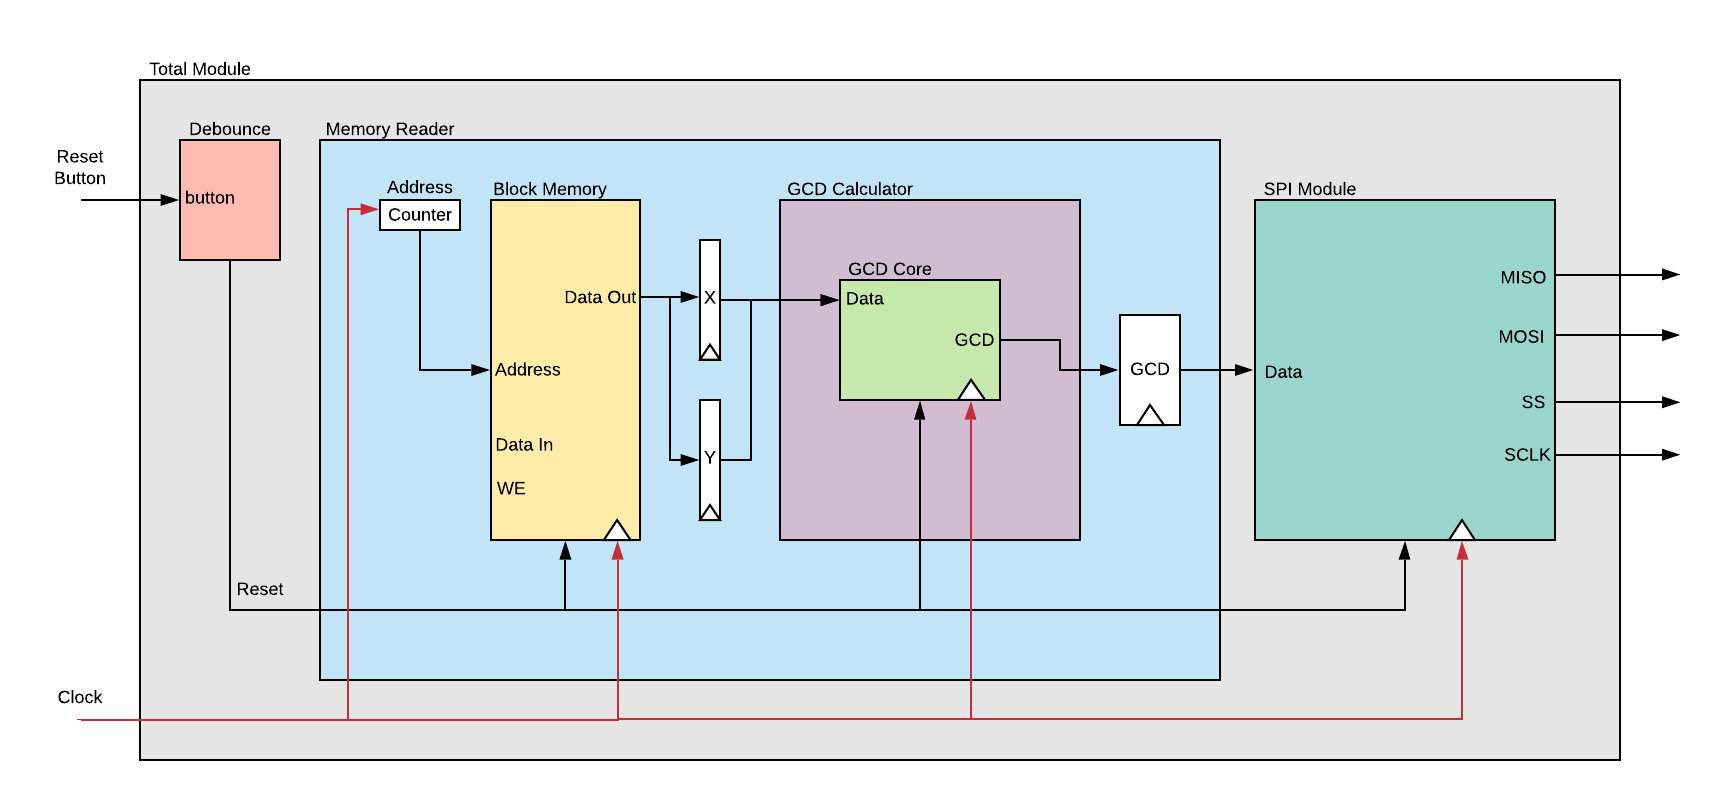
\includegraphics[width=1.1\textwidth]{BD.png}
\caption{Block Diagram of my approach to Project \#5.}
\label{fig:behav-sim}
\end{figure}

For simplicity, I did not show all connections to registers, nor the modules within the GCD core. Also, \textit{WE} and \textit{Data In} are not shown to be connected, but they are internally unused (grounded) as no writing to the block memory is utilized.

My approach to the project will be to create a memory reader module that interacts with the block memory unit, reading the pairs of data one at a time (one pair at a time), and then interacting with the GCD module through a GCD wrapper of sorts. This wrapper will take the X and Y data and interact with the GCD with the required timing, sending the final GCD result back to the memory reader module. Once this has been done for the current pair, the GCD data will be sent to an SPI module that implements the SPI protocol that serves as an output for the total module. This will be repeated for each pair of data read in the block memory, until the memory reader identifies a zero.

The SPI module will utilize a parameterized \textit{down-clocking} of sorts, where a specified count $x$ can be given, and each $x$ clock pulses, the SPI FSM will increment - allowing for easily configured timing of SCLK, without the need for dummy states within the FSM.

Of course, when implemented on hardware, this will utilize the debounce module to reset all modules and registers within the circuit.

\end{document}